% !TEX spellcheck = en_US

The steady states are influenced by the design of the controller and turbine.
The static behavior in every operating point can be shown by the calculation of steady states.
Such calculated steady states provide an crucial overview of the turbines behavior early in the design process.
Additionally, these steady states play a important role in the overall wind turbine design and can be utilized to initialize further simulations.

The general procedure we followed to find the steady-state parameters is as follows: 
\begin{enumerate}
	\item Determine the wind speeds for the control regions. 
	\item Calculate the steady states below the rated wind speed separately for regions 1, 1.5, 2, and 2.5. With the determined wind speeds from step 1.
	\item Calculate the steady states above the rated wind speed.
\end{enumerate}

With the help of the differential equation \ref{eq:omega dot} for the rotor motion the steady states are derived.

\begin{equation}
	\dot{\Omega} = \frac{M_a(v_0, \Omega, \theta) - M_G}{J}
	\label{eq:omega dot}
\end{equation}

The condition to reach a steady state is $\dot{\Omega} = 0$. The determined parameter is the variable and the other parameters are fixed. The conditions to which are the fixed parameters set are depending on the control region hence the behavior of the turbine itself.

%Find $v_{rated}$, $v_{1to1.5}$, $v_{1.5to2}$ and $v_{2to2.5}$ using the minimization problem method, as shown in \ref{equation:Minimization problem}. 
%Additionally, use the minimization problem method to determine the above-rated wind speed, as shown in Equation \ref{equation:Minimization problem above rated wind}.
%
%\begin{equation}
%	\min_{v_0} \left( M_a(v_0, \Omega, \theta) - M_G \right)^2
%	\label{equation:Minimization problem}
%\end{equation}
%
%
%\begin{equation}
%	\min_{\theta} \left( M_a(v_0, \Omega, \theta) - M_G \right)^2
%	\label{equation:Minimization problem above rated wind}
%\end{equation}

In the \gls{shakti} simulation model, simulations are performed for wind speeds ranging from 3 to 25 m/s.
The steady state values for wind speed, pitch angle, rotor speed, tip speed ratio, power coefficient, generator torque and tower top displacement are derived by \ref{eq:omega dot}.
Additionally, the results are visually assessed through plots.
The wind speeds of the control regions are $v_{rated} = 9.3531$, $v_{1to1.5} = 6.0652$, $v_{1.5to2} = 6.0652$ and $v_{2to2.5} = 8.6631$. Figure \ref{fig:power cureve} demonstrates the model's power curve.

\begin{figure}[h]
	\centering
	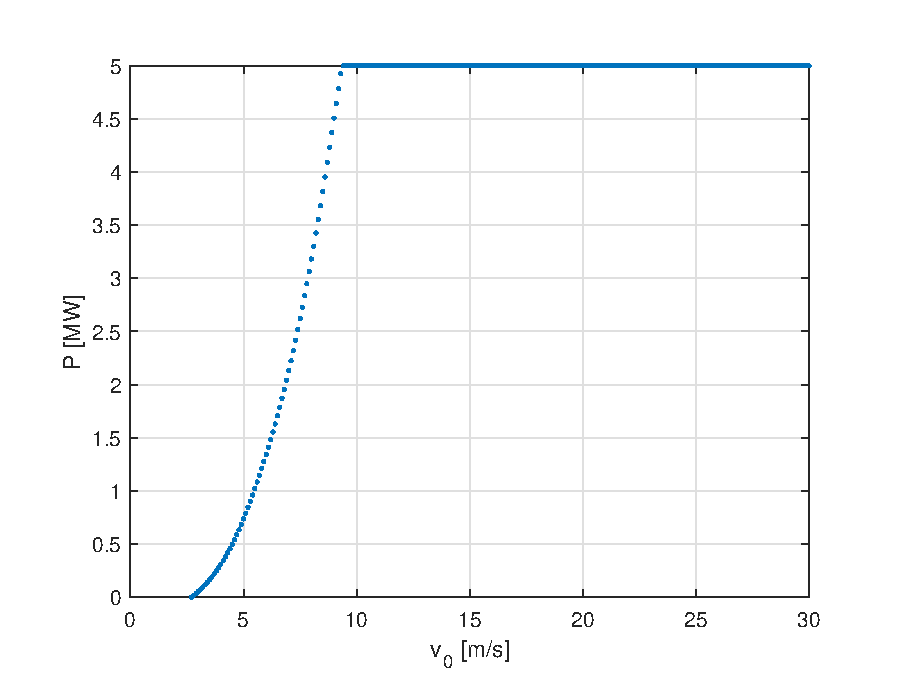
\includegraphics[width=0.7\textwidth]{Figures/P_Vs_v.eps}
	\caption{Power curve calculated with steady state calculations}
	\label{fig:power cureve} 
\end{figure}
